\chapter{I referti medici}
\section{La struttura dei referti}
I referti prodotti nei laboratori del policlinico seguono la struttura standard adottata dall'Azienda Tutela Salute Sardegna (dal 2022 Azienda Regionale della Salute, ARES) 
presentando una divisione in 4 blocchi:
Se sono presenti più analisi, o le informazioni dell'analisi superano una certa quantità (per esempio un antibiogramma molto lungo) il documento viene suddiviso su più pagine.
Di norma i referti prodotti non superano le due pagine.

\begin{center}
	\begin{itemize}
		\item Intestazione ATS
		\item Sezione anagrafica
		\item Contenuto referto
		\item Piè di pagina
		\end{itemize}
\end{center}
\par\bigskip
\subsection{L'intestazione ATS}
Il primo blocco, contenente l'intestazione, identifica la provenienza del documento mostrando informazioni sull'ASL quali strutture ad essa collegate, i recapiti telefonici e il logo.
\begin{figure}[h!]
	\centering
	
\includegraphics[width=.99\columnwidth]{images/header.png}
	\caption{\textit{Intestazione iniziale di un referto}}
	\label{fig:header}
\end{figure}
\bigskip

\subsection{La sezione anagrafica}
Segue la sezione anagrafica che indica la priorità dell'analisi effettuata, la provenienza del paziente (intesa come reparto di provenienza) e le informazioni personali del paziente.
\begin{figure}[h!]
	\centering
	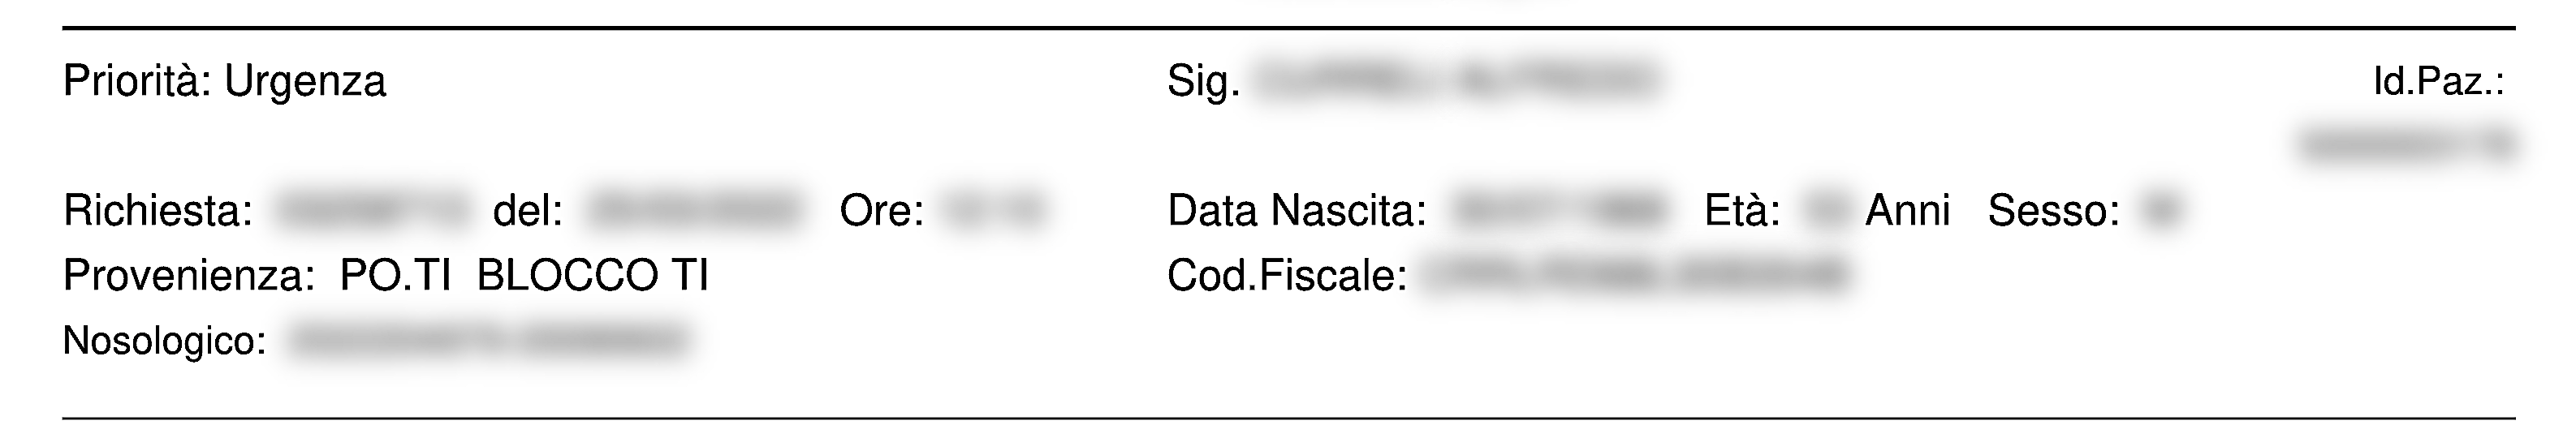
\includegraphics[width=.99\columnwidth]{images/sezione_anagrafica.png}
	\caption{\textit{Sezione anagrafica che mostra la priorità e le informazioni sul paziente}}
	\label{fig:header}
\end{figure}
\bigskip
\subsection{Il contenuto del referto}
Al centro è collocato il risultato dell'analisi, che varia a seconda dell'obbiettivo del test, l'implementazione attuale è progettata per trovare ed estrarre le tabelle antibiogramma. Un esempio di contenuto valido per l'estrazione è quello della \ref{fig:content}
\begin{figure}[h!]
	\centering
	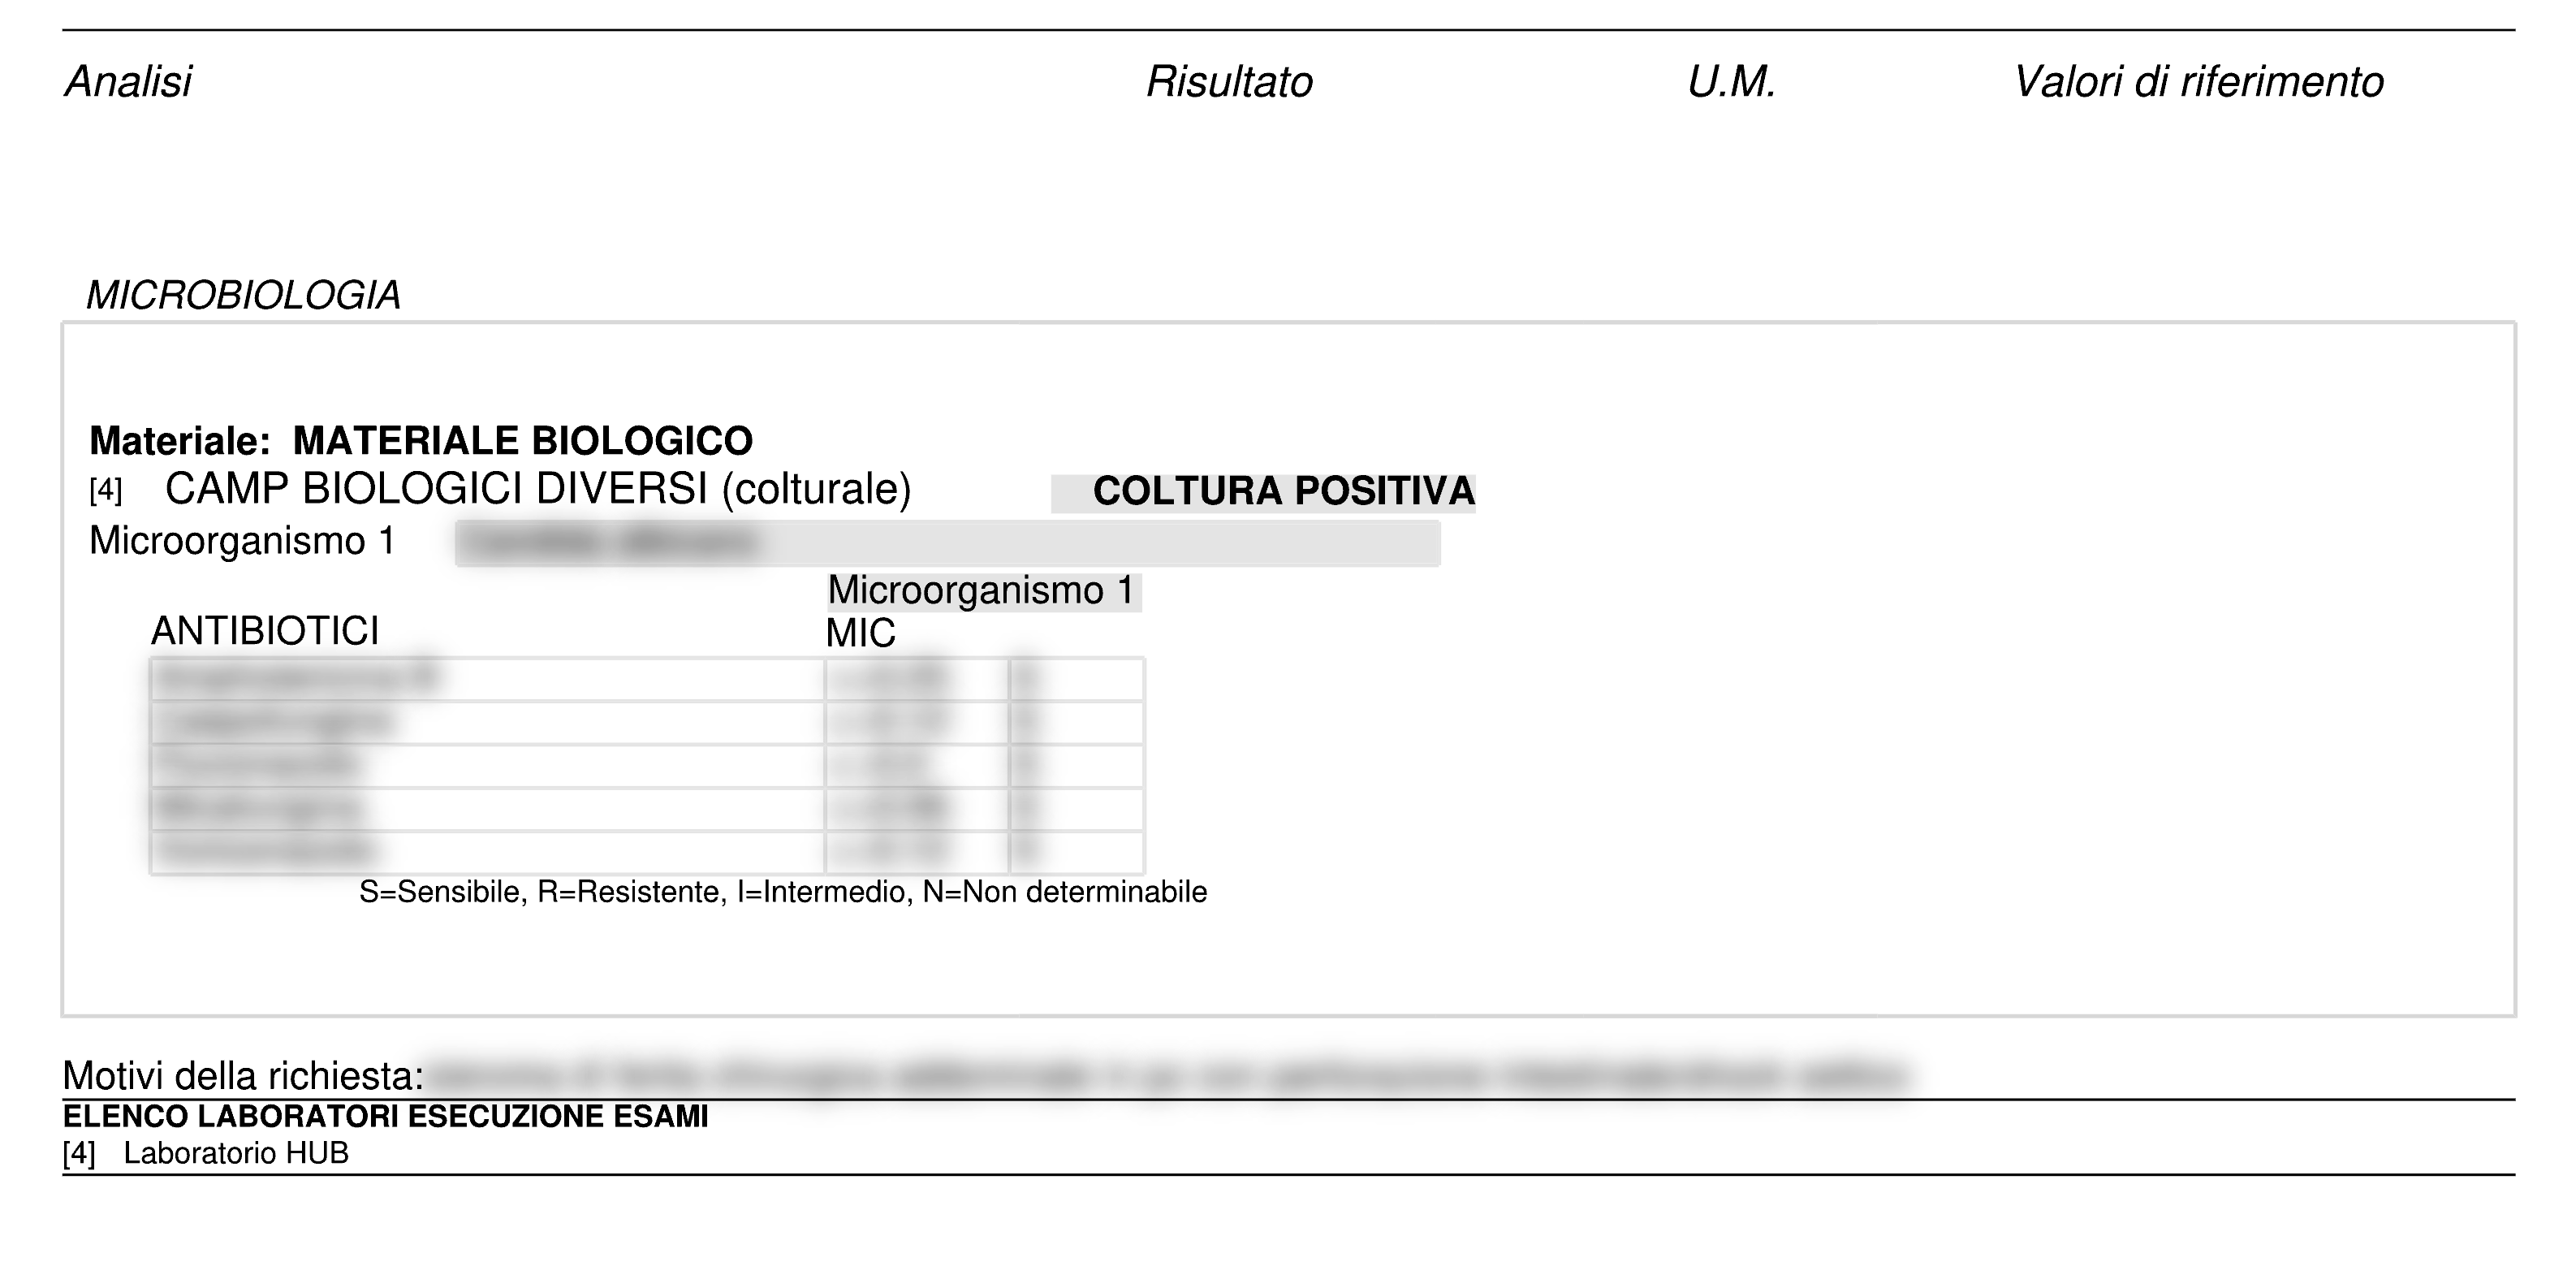
\includegraphics[width=.99\columnwidth]{images/content.png}
	\caption{\textit{miao}}
	\label{fig:content}
\end{figure}
\bigskip
\newpage
\subsection{Il piè di pagina}
Infine, nel
\begin{figure}[h!]
	\centering
	
\includegraphics[width=.99\columnwidth]{images/footer.png}
	\caption{\textit{Piede di pagina}}
	\label{fig:content}
\end{figure}
\bigskip


\section{Tipologie di referti}
Nell'ambito di questa tesi possiamo distinguere 5 tipologie di referti a seconda del loro contenuto:
\begin{itemize}
	\item Singolo Antibiogramma
	\item Antibiogramma multiplo
	\item Antibiogramma singolo multi-pagina
	\item Antibiogramma multiplo multi-pagina
	\item Referto senza tabelle
\end{itemize}
